\documentclass[a4paper,11pt,twocolumn]{article}

% gap of colummns
\setlength{\columnsep}{.5cm}

% fonts
\usepackage[utf8]{inputenc}
%\usepackage[francais]{babel}

% to get hyphenation on accented words
\usepackage[T1]{fontenc}

% href
\usepackage{hyperref}
\hypersetup{
    colorlinks=true,
    linkcolor=blue,
    filecolor=blue,      
    urlcolor=blue,
    bookmarks=true
}

% quotes
\usepackage{csquotes}

% code highlighting
\usepackage{minted}
\usemintedstyle{pastie}

% asm
\usepackage{amsmath}
\usepackage{amssymb}
\usepackage{amsthm}

% inline code
\usepackage{listings}
\usepackage{xcolor}

% tables
\usepackage{booktabs}

% algorithm
\usepackage[]{algorithm2e}

% for right cases
\newenvironment{rcases}
  {\left.\begin{aligned}}
  {\end{aligned}\right\rbrace}
  
% images
\usepackage{graphicx}
\usepackage{float}

% diagrams
\usepackage{tikz}
\usetikzlibrary{matrix}
\usetikzlibrary{positioning}

% tables
\usepackage{booktabs}

% no identation
\setlength{\parindent}{0pt}

% theorem
\newtheorem{definition}{Definition}
\newtheorem{property}{Property}
\newtheorem{theorem}{Theorem}

% header
\title{How to Backdoor Diffie-Hellman}
\author{David Wong}
\date{\emph{NCC Group}, \small{March 2016}}

% notes
\usepackage[draft]{todonotes}
\setlength{\marginparwidth}{2cm}

% 
\begin{document}
\maketitle
\renewcommand{\abstractname}{Abstract}
\begin{abstract}
Lately several backdoors in cryptographic constructions, protocols and implementations have been surfacing in the wild. Dual-EC in RSA's B-Safe product, A modified Dual-EC in Juniper's operating system ScreenOS and a non-prime modulus in the Socat open-source tool. The question on how fragile cryptographic constructions are if we do not use Nothing-Up-My-Sleeve numbers has came up in many papers, but the question on how to introduce a backdoor in an already secure, safe and easy to audit implementation has so far never been researched (in the public).\\
In this work we present two ways of building a Nobody-But-Us Diffie-Hellman backdoor with a composite modulus and a hidden subgroup (CMHS) and with a composite modulus and a smooth order (CMSO). We then explain how we subtly implemented it and exploited it in various open source libraries using the TLS protocol.\\
\\
\textbf{Keywords:} Diffie-Hellman, Ephemeral, DHE, NOBUS, backdoor, Discrete Logarithm, Small subgroup attack, Pohlig-Hellman, Factorization, Pollard's p-1 algorithm, ECM, Dual EC, Juniper, Socat\\

\end{abstract}
\section{Introduction}\label{introduction}

Around Christmas 2015, a company named \emph{Juniper} released an \href{https://kb.juniper.net/InfoCenter/index?page=content&id=JSA10713&actp=search}{out of cycle security bulletin}. Two vulnerabilities were being semi-disclosed, without much details to help us grasp the seriousness of the situation. Fortunately, at this period of the year many researchers were home with nothing else to do but to try solving this puzzle. Quickly, by diffing both the patched and vulnerable binaries, the two issues were pinpointed. While one of the vulnerability was a simple ``master''-password implemented at a crucial step of the product's authentication, the other discovery was a bit more subtle: a unique value was modified. More accurately, a number was replaced. The introduction of the vulnerability was so trivial that the simple use of the unix command line tool \mintinline{bash}{strings} was enough to discover the change.

\begin{figure}[H]
\centering
\includegraphics[width=\columnwidth]{patched_bin.png}
\caption{The strings of the patched binary}\label{screenOS}
\end{figure}

\begin{figure}[H]
\centering
\includegraphics[width=\columnwidth]{vulnerable_bin.png}
\caption{The strings of the vulnerable binary}\label{screenOS}
\end{figure}

Behind that modified number was hiding a \emph{Dual EC} value. Dual EC is a Pseudo-Random Number Generator (PRNG) that is believed to have been backdoored by the NSA \cite{dualEC}. The PRNG's core has the ability to provide a Nobody But Us (NOBUS) trapdoor: a secret passage that can only be accessed by the people holding the secret key. In our case: the elliptic curve discrete logarithm $k$ in the Dual EC equation $Q = [k]P$ (where $P$ and $Q$ are the two elliptic curve points used in the foundation of Dual EC).\\

Although the quest to find the Juniper's backdoor and the numerous open questions that arose from that work are a fascinating read by itself \cite{juniper}, it is only the introduction of this work that aims to show how secure and strong cryptographic constructions are a simple and subtle change away from being your own secretive pipe-show.\\

On February the 1st 2016, only a few months after Juniper's debacle, \emph{Socat} \href{http://www.openwall.com/lists/oss-security/2016/02/01/4}{published a security advisory of its own}.

\begin{displayquote}
In the OpenSSL address implementation the hard coded 1024 bit DH p parameter was not prime. The effective cryptographic strength of a key exchange using these parameters was weaker than the one one could get by using a prime p. Moreover, since there is no indication of how these parameters were chosen, the existence of a trapdoor that makes possible for an eavesdropper to recover the shared secret from a key exchange that uses them cannot be ruled out.
\end{displayquote}

\todo{this is irrelevant, change that part. Also I should explain here that DHE is interesting to backdoor because unlike RSA, DH, ECDH, ... people use the default parameters of libraries/products and don't generate their own in a certificate}In the same vein of Juniper's problem, a single number was changed. But Socat's problems root deeper. A year before that suspicious 1024 bit Diffie-Hellman (DH) value was introduced, the free software would have served its TLS connection using a 512 bit DH modulus. The problem with such small DH parameters is already well known \cite{logjam}, in the paper the authors point out that most servers use common Diffie-Hellman parameters to generate their ephemeral Diffie-Hellman key exchanges, they point that the problem is that they are 1024bits which the NSA might be able to crack. This initiated a debate on how users should use Diffie-Hellman, should they generate their own DH parameters or use predefined parameters that RFC \todo{list the rfc with the DH groups} or libraries use by default? The problem of implementing DH securely are unfortunately rarely well understood as well. The defense approach is told in several RFCs \cite{rfc2631} \cite{rfc2785}, but no paper so far take the point of view of the attacker.\\

\todo{redo all that part}In section 2, we will first discard some possible mistakes that the troublemaker could have made. In section 3 we will introduce the different attacks available on DH, from small subgroup attacks to Pohlig Hellman's algorithm. We will start by explaining how to implement a NOBUS backdoor in Diffie-Hellman in section 4, and we will follow with the bulk of our contribution in section 5: that is the different methods to achieve that goal. In section 6 we will see what's wrong with the previous methods, and use what we learned from that to try to reverse Socat's 1024 bit DH modulus. Informationally, we will test the security of the new 2048 bit DH modulus of Socat in section 7, and follow by brief explanations on how to secure a DH implementation. Eventually we will wrap it all in section 9.

\section{Attacks on Diffie-Hellman and the Discrete Logarithm}

To attack a Diffie-Hellman key exchange, the attacker needs to extract the secret key $a$ from one of the peer's public key $y_a = g^a \pmod{n}$. He can then compute the shared key $g^{ab} \pmod{n}$ using the other peer's public key $y_b = g^b \pmod{n}$.\\

The naive way to go about this is to compute each power of $g$ (while tracking the exponent) until the public key is found. This is called \emph{trial multiplication} and would need on average $\frac{n}{2}$ operations to find a solution.
More efficiently, algorithms that compute discrete logarithm in expected $\sqrt{q}$ steps (with $q$ the order of the base) like Baby-step-giant-step (deterministic), Pollard rho or Pollard Kangaroo (both probabilistic) can be used. Because of the space required for Baby-step-giant-step, Pollard's algorithms are often preferred. While both are parallelizable, Kangaroo is used when the order is unknown or known to be in a small interval. For bigger groups the Index Calculus or other Number Field Sieve (NFS) algorithms are the most efficients. But so far, computing a discrete logarithm in polynomial time on a classical computer is still an open problem.\\

\subsection{Pollard Rho}

The algorithm that interests us here is Pollard Rho: it is fast in relatively small orders, it is parallelizable and it takes very little amount of memory to run. The idea comes from the Birthday Paradox and that equation (where $x$ is the secret key we are looking for):
\begin{align*}
  g^{xa +b } = g^{xa' + b'} \pmod{p}&\\
  \implies x = (a-a')^{-1} (b' - b) \pmod{p-1}&
\end{align*}
The birthday paradox tells us that by looking for a random collision we can quickly find one in $\mathbb{O}(\sqrt{n})$. A random function is used to efficiently step through various $g^{xa + b}$ until two values repeat themselves, it is then straightforward to calculate $x$. Cycle-finding algorithms are used to avoid storing every iterations of the algorithm (Two different iterations of $g^{xa+b}$ are started and end up in a loop passed a certain step) and the technique of distinghuished points is used to parallelize the algorithm (paralleled machines only save and share particular iterations, for example iterations starting with a chosen number of zeros).

\subsection{Pohlig-Hellman}

In 1978, Pohlig and Hellman discovered a shortcut to the discrete logarithm problem\footnote{S. Pohlig and M. Hellman "\href{http://www-ee.stanford.edu/~hellman/publications/28.pdf}{An Improved Algorithm for Computing Logarithms over GF(p) and its Cryptographic Significance}"}\cite{PH}: if you know the complete factorization of the order of the group, and all of the factors are relatively small, then the discrete logarithm can be quickly computed.

The idea is to find the value of the secret key $x$ modulo the divisors of the group's order by reducing the public key $y = g^x \pmod{n}$ in subgroups of order dividing the group order. Thanks to the Chinese Remainder Theorem (CRT) stated later, the secret key can then be reassembled in the group order. Summed up below is the full Pohlig-Hellman algorithm:

\begin{enumerate}
    \item Determine the prime factorization of the order of the group
        $$\varphi(n) = \prod p_i^{k_i} $$
    \item Determine the value of $x$ modulo $p_i^{k_i}$ for each $i$
    \item Recompute $x \pmod{\varphi(n)}$ with the CRT
\end{enumerate}

The ruse of Pohlig-Hellman's algorithm is in how do we determine the value of the secret key $x$ modulo each factor $p_i^{k_i}$ of the order. One way of doing it is to try to reduce our public key to the subgroup we're looking at by computing:
$$y^{\varphi(n)/p_i^{k_i}} \pmod{n}$$
Computing the discrete logarithm of that value, we get $x \pmod{p_i^{k_i}}$. This works because of the following observation (note that $x$ can be written $x_1 + p_i^{k_i} x_2$ for some $x_1$ and $x_2$):
\begin{align*}
    y^{\varphi(n)/p_i^{k_i}} &= (g^{x})^{\varphi(n)/p_i^{k_i}} \pmod{n}\\
    &= g^{(x) \varphi(n)/p_i^{k_i}} \pmod{n}\\
    &= g^{(x_1 + p_i^{k_i} x_2) \varphi(n)/p_i^{k_i}} \pmod{n}\\
    &= g^{x_1 \varphi(n)/p_i^{k_i}} g^{x_2 \varphi(n)} \pmod{n}\\
    &= g^{x_1 \varphi(n)/p_i^{k_i}} \pmod{n}\\
    &= g^{(\varphi/p_i^{k_i})^{x_1}}
\end{align*}
The value we obtain is a generator of the subgroup of order $p_i^{k_i}$ raised to the power $x_1$. By computing the discrete logarithm of this value, we will obtain $x_1$ which is the value of $x$ modulo $p_i^{k_i}$. Generally we will use Pollard Rho to do that.\\

The Chinese Remainder Theorem, sometimes used for the good \footnote{ Shinde, Fadewar \href{http://www.techscience.com/doi/10.3970/icces.2008.005.255.pdf}{Faster RSA Algorithm for Decryption Using Chinese Remainder Theorem}}\cite{fasterRSA} will be of use here for the bad. The following theorem states why it is possible for us to find a solution to our problem once we found a solution modulo each power prime factor of the order.

\begin{theorem}
Suppose $m = \prod\limits^{k} m_i$ with $m_1, \cdots, m_k$ pairwise co-prime.\\

For any $(a_1, \cdots, a_k)$ there exists a $x$ such that:
$$
\begin{cases}
x= a_1 \pmod{m_1}\\
\vdots\\
x= a_k \pmod{m_k}\\
\end{cases}\\
$$

And there exist a unique solution for $x \pmod{m}$
\end{theorem}

There is a simple way to recover the $x \pmod{m}$ which we will use to later reconstruct the secret key modulo the order of the group.
\begin{proof}
  \begin{align*}
      x &= \sum^{k} a_i * (\prod_{j \neq i} m_{j} \overline{m}_{j}) \pmod{m} \\
      \mbox{with }\overline{m}_{j} &= m_{j}^{-1} \pmod{m_i}
  \end{align*}
\end{proof}
At first, it might be kind of hard to grasp where that formula is coming from. But let me explain by starting with only two equations. Keep in mind that we want to find the value of $x$ modulo $m = m_1 m_2$
\[
\begin{rcases}
x = a_1 \pmod{m_1}\\
x = a_2 \pmod{m_2}
\end{rcases}
\implies x = \text{ ?} \pmod{m}
\]\\
How can we start building the value of $x$?
\begin{align*}
&\text{If } x = a_1  m_2\pmod{m} \text{,}\\
&\text{then }
\begin{cases}
x = \boldsymbol{a_1} m_2 \pmod{m_1}\\
x = \boldsymbol{0} \pmod{m_2}\\
\end{cases}
\end{align*}

Quite not what we want, but we are getting there. Let's add to it:
\begin{align*}
%\begin{aligned}
&\text{If } x = a_1  m_2 \overline{m}_2 \pmod{m}\\
&\overline{m}_2 \text{ the integer congruent to } m_2^{-1} \pmod{m_1}\\
&\text{then } \begin{cases}
    x = a_1 m_2 \overline{m}_2 = \boldsymbol{a_1} \pmod{m_1}\\
x = 0 \pmod{m_2}\\
\end{cases}
\end{align*}
That's almost what we want! Half of what we want actually. We just need to do the same thing for the other side of the equation, and we have:
\begin{center}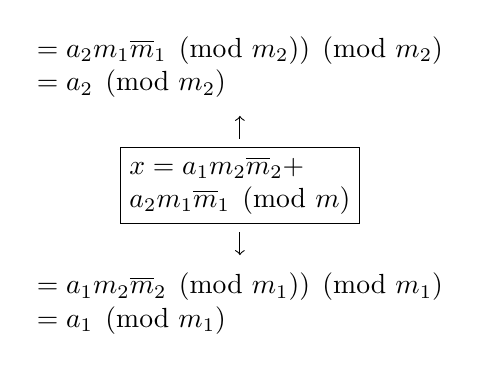
\begin{tikzpicture}[scale=.55]
% main formula
  \node[align=left, draw] (main) {$x = a_1 m_2 \overline{m}_2 +$\\
    $a_2 m_1 \overline{m}_1 \pmod{m}$};
% other formulas
\node (formula1) [below=.5cm of main, align=left] {$= a_1 m_2 \overline{m}_2 \pmod{m_1}) \pmod{m_1}$\\$= a_1 \pmod{m_1}$};
\node (formula2) [above=.5cm of main, align=left] {$= a_2 m_1 \overline{m}_1 \pmod{m_2}) \pmod{m_2}$\\$= a_2 \pmod{m_2}$};
% arrows
\draw [->, shorten <=3pt, shorten >=3pt] (main) -- (formula1);
\draw [->, shorten <=3pt, shorten >=3pt] (main) -- (formula2);
\end{tikzpicture}\end{center}
with $\overline{m}_2$ the integer congruent to $m_2^{-1} \pmod{m_1}$ and $\overline{m}_1$ the integer congruent to $m_1^{-1} \pmod{m_2}$.\\

Everything works as we wanted! Now you should understand better how we came up with that general formula. There has been improvement to it with the Garner's algorithm but this method is so fast anyway that it is not the bottleneck of the whole attack.\todo{ref for garner}

\subsection{Small Subgroup Attacks}

The attack we just visited is a passive attack: the knowledge of one Diffie-Hellman exchange between two parties is enough to obtain the following shared key. But instead of reducing one party's public key to an element of different subgroups, there is another clever attack called a small subgroup attack that creates the different subgroup generators directly and send them to one peer successively to obtain his private key. It is an active attack that doesn't work against certain ephemeral protocols that renew the Diffie-Hellman public key for every new key exchange. This is for example the case of certain implementations of TLS when using ephemeral Diffie-Hellman (DHE) as a key exchange during the handshake. This variant of Diffie-Hellman allows for \emph{Perfect Forward Secrecy}, a mode that protects against decryption of past and future communications in case the long-term private key is stolen.

The attack is pretty straight forward and summed up below:

\begin{enumerate}
    \item Determine the prime factorization of the order of the group
      $$\varphi(n) = \prod p_i^{k_i} $$
    \item Find a generator for every subgroup of order $p_i^{k_i}$, this can be done by picking a random element $\alpha$ and computing
      $$g = \alpha^{\frac{order}{p_i^{k_i}}}$$
    \item Send generators one by one as your public keys in different key exchanges
    \item Determine the value of $x$ modulo $p_i^{k_i}$ for each shared key computed
    \item Recompute $x \pmod{\varphi(n)}$ with the CRT
\end{enumerate}

The fourth step can be done by having access to an Oracle telling you what is the shared key computed by the victim. In TLS this is done by brute-forcing the possible solutions and seeing which one has been used by the victim in his following encrypted messages (for example the MAC computation in the Finish message during the handshake). In this settings the attack would be weaker than Pohlig-Hellman since the brute-force is slower than Pollard Rho, or even trial multiplication. Because of the previous limitations and the fact that this attacks only works for rather small subgroups we won't use it in this work.

\section{A First Backdoor Attempt in Prime Groups}

The naive approach would be to weaken the parameters enough to make the computation of discrete logarithms affordable. Making the modulus a prime of a special form ($r^e + s$ with small $r$ and $s$) would facilitate the Special Number Field Sieve (SNFS) algorithm. Having a small modulus would also allow for easier pre-computation of the General Number Field Sieve (GNFS) algorithm. In [\todo{need ref}logjam] it is believed that the NSA has enough power to achieve the first pre-computing phases of GNFS on 1024bits prime which would then allow them to compute discrete logarithms in such large primes in the matter of seconds. But these ideas are pure computational advantages that involve no secret key to make the use of efficient backdoors possible. Moreover they are downright not practical: the attacker would have to re-do the pre-computing phase entirely for every different modulus, and the next generation of recommended modulus bitsize (2048+) would make these kind of computational advantages fruitless. Another approach could be to use a generator of a smaller subgroup (without publishing what smaller subgroup we use) so that algorithms like Pollard Rho would be cost-effective again.

\begin{center}
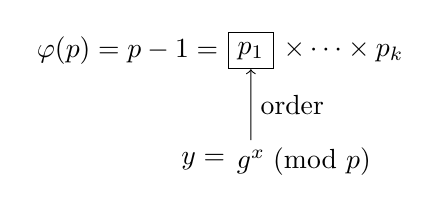
\begin{tikzpicture}[scale=.55]
% main formula
  \node (order) {$\varphi(p) = p-1 = $};
  \node (small) [draw,right=0cm of order] {$p_1$};
  \node [right=0cm of small] {$\times \cdots \times p_k$};
  % first line
  \node (g) [below=.9cm of small, align=left] {$g^x$};
  \node [left=-.1cm of g] {$y=$};
  \node [right=-.3cm of g] {$\pmod{p}$};
% arrows
\draw [->] (g) -- (small) node [midway,right] {order};
\end{tikzpicture}
\end{center}

But then algorithms like Pollard Kangaroo that run in the same amount of time as Pollard Rho and that do not require the knowledge of the base's order could be used as well by anyone willing to try. This makes it a poorly hidden backdoor that we cannot qualify as NOBUS\todo{do we have a clear definition of NOBUS?}.

Our first contribution (CM-HSS) in section 4 makes both of these ideas possible by using a composite modulus. GNFS and SNFS can then be used modulo the factors of the composite modulus, or the generator's ``small'' subgroups can be concealed modulo the factors as well.\\

A second idea would be to set the scene for the Pohlig-Hellman algorithm to work. This can be done by fixing a prime modulus $p$ such that $p-1$ is B-smooth \todo{definition of B-smooth, should include it in the previous section tho} with B small enough for discrete logarithms in bases of order B to be possible.\\

\begin{center}
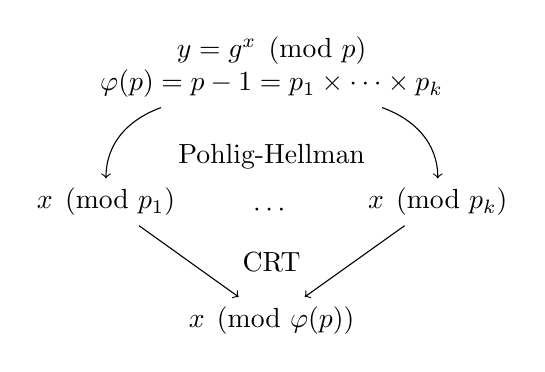
\begin{tikzpicture}[scale=.55]
% main formula
\node[align=center] (main) {$y = g^x \pmod{p}$\\
$\varphi(p) = p-1 = p_1 \times \cdots \times p_k$};
% first line
\node (xmodp1) [below left=.9cm and -1.2cm of main, align=left] {$x \pmod{p_1}$};
\node (dots) [below=1.1cm of main, align=left] {$\cdots$};
\node (xmodpk) [below right=.9cm and -1.2cm of main, align=left] {$x \pmod{p_k}$};
% Pohlig Hellman
\node (PH) [above=.2cm of dots, align=left] {Pohlig-Hellman};
% arrows
\draw (main) edge[out=200,in=90,->] (xmodp1);
\draw (main) edge[out=340,in=90,->] (xmodpk);
% second line
\node (xmodpm1) [below=.9cm of dots, align=left] {$x \pmod{\varphi(p)}$};
% CRT
\node (CRT) [above=.2cm of xmodpm1, align=left] {CRT};
% arrows
\draw [->] (xmodp1) -- (xmodpm1);
\draw [->] (xmodpk) -- (xmodpm1);
\end{tikzpicture}
\end{center}

But this design is flawed in the same ways as the previous ones were: anyone can compute the order of the group ($p - 1$) and try to factor it. Anything below 300bits\todo{where does that number comes from?? show some ref} is relatively easy to factor using the \emph{Elliptic Curve Method} (ECM), a factorization algorithm which complexity only depends on the largest factor. This lower bound on the factors make it impossible for us to use our $\mathbb{O}(\sqrt{p-1})$ algorithm which would take more than $2^{150}$ operations to solve the discrete logarithm of such orders. \\

Our second contribution in section 5 uses a composite modulus to hide the smoothness of the order (CM-HSO) as long as the modulus cannot be factored. This method is preferred from the first contribution as it might only need a change of modulus. For example, in many DH parameters or implementations, $g=2$ as a generator is often used. While our first contribution will not allow any easy ways to find a specific generator, our second method will.

\section{A composite modulus for a NOBUS backdoor with a hidden subgroup(CM-HSS)}

Let's think at our first idea in the previous section, but this time using a composite modulus $n=pq$. The discrete logarithm problem can be reduced modulo $p$ and $q$ and solved there before being reconstructed modulo $pq$ with the CRT.\todo{have we stated the abbreviation before?}

\begin{center}
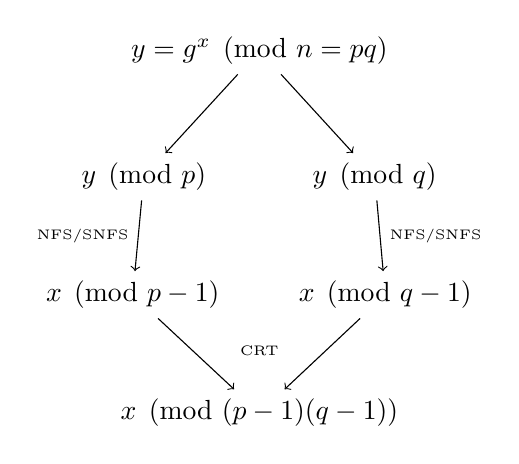
\begin{tikzpicture}
% main formula
\node[align=center] (main) {$y = g^x \pmod{n=pq}$};
% first line
\node (ymodp) [below left=1cm and -1.2cm of main, align=left] {$y \pmod{p}$};
\node (ymodq) [below right=1cm and -1.2cm of main, align=left] {$y \pmod{q}$};
% arrows
\draw [->] (main) -- (ymodp);
\draw [->] (main) -- (ymodq);
% second line
\node (xmodpm1) [below left=.9cm and -2cm of ymodp, align=left] {$x \pmod{p-1}$};
\node (xmodqm1) [below right=.9cm and -2cm of ymodq, align=left] {$x \pmod{q-1}$};
% arrows
\draw [->] (ymodp) -- (xmodpm1) node[midway, left] {{\tiny NFS/SNFS}};
\draw [->] (ymodq) -- (xmodqm1) node[midway, right] {{\tiny NFS/SNFS}};
% CRT
\node (CRT) [below=4cm of main, align=left] {$x \pmod{(p-1)(q-1)}$};
\node [above=0.3cm of CRT, align=left] {{\tiny CRT}};
% arrows
\draw [->] (xmodpm1) -- (CRT);
\draw [->] (xmodqm1) -- (CRT);
\end{tikzpicture}
\end{center}

$p$ and $q$ could be hand-picked as SNFS primes, or we could use GNFS to compute the discrete logarithm modulo $p$ and $q$. But a more efficient way exists that allow us to reduce algorithms like Pollard Rho dramatically. By fixing a generator that modulo $p$ and $q$ generates a ``small'' subgroup, we would just need to compute two discrete logarithms in two small subgroups instead of one discrete logarithm in one large group. For example, we could pick $p$ and $q$ such that $p-1 = 2p_1p_2$ and $q-1=2q_1q_2$ with $p_1$ and $q_1$ two small prime factors and $p_2, q_2$ two large prime factors. Lagrange's theorem tells us that the possible order of the subgroups are divisors of the group order. This mean we can probably find an element $g$ of order $p_1q_1$ to be our Diffie-Hellman generator.

\begin{center}
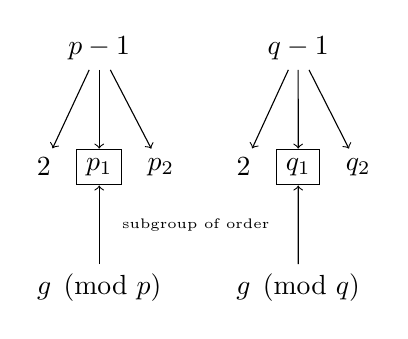
\begin{tikzpicture}[scale=.55]
% pm1
\node (pm1) {$p-1$};
\node (pm1_small) [draw, below=1cm of pm1] {$p_1$};
\node (pm1_2) [left=.2cm of pm1_small] {$2$};
\node (pm1_big) [right=.2cm of pm1_small] {$p_2$};

\draw [->] (pm1) -- (pm1_2);
\draw [->] (pm1) -- (pm1_small);
\draw [->] (pm1) -- (pm1_big);

\node (gmodp) [below=1cm of pm1_small] {$g \pmod{p}$};
\draw [->] (gmodp) -- (pm1_small) node [midway, right] {{\tiny \space\space subgroup of order}};

% pm2
\node (qm1) [right=1.5cm of pm1] {$q-1$};
\node (qm1_small) [draw, below=1cm of qm1] {$q_1$};
\node (qm1_2) [left=.2cm of qm1_small] {$2$};
\node (qm1_big) [right=.2cm of qm1_small] {$q_2$};

\draw [->] (qm1) -- (qm1_2);
\draw [->] (qm1) -- (qm1_small);
\draw [->] (qm1) -- (qm1_big);

\node (gmodq) [below=1cm of qm1_small] {$g \pmod{q}$};
\draw [->] (gmodq) -- (qm1_small);
\end{tikzpicture}
\end{center}

By reducing the discrete logarithm problem $y = g^x$ modulo $p$ and $q$ with our new backdoored generator, we can compute $x$ modulo $p-1$ and $q-1$ more easily and then recompute an equivalent secret key modulo $(p-1)(q-1)$. This will find the original secret key with a probability of $\frac{1}{4p_2q_2}$ which is tiny, but it doesn't matter since the shared key we will compute with that solution and the other peer's public key will be the valid shared key. This is because of the following:
\begin{proof}
Let $a + k_ap_1q_1$ be Alice's public key for $k_a \in \mathbb{Z}$ and let $b + k_bp_1q_1$ be Bob's public key for $k_b \in \mathbb{Z}$,\\
then Bob's shared key will be $(g^{a+k_ap_1q_1})^{b+k_bp_1q_1} = g^{ab} \pmod{n}$.\\
Let $a + k_cp_1q_1$ be the solution we found for $k_c \in \mathbb{Z}$,\\
then the shared key we will compute will be $(g^{b+k_bp_1q_1})^{a+k_cp_1q_1} = g^{ab}\pmod{n}$ which is the same as Bob's shared key.
\end{proof}
We used the Pollard Rho function in Sage 6.10 on a macbook pro with an i7 Intel Core @ 3.1GHz to compute discrete logarithms modulo safe primes of diverse bitsizes. The results are summed up in the table below.

\begin{center}
  \begin{tabular*}{\columnwidth}{@{} c  @{\extracolsep{\fill}} cc @{}}
    \toprule
    order size & expected complexity & time \\
    \midrule
    40 bits & 2^{20} & 01s \\
    45 bits & 2^{22} & 04s \\
    50 bits & 2^{25} & 34s \\
    \bottomrule
  \end{tabular*}
\end{center} 

A stronger and more clever attacker would parallelize this algorithm on more powerful machines to obtain better numbers. To be able to exploit the backdoor ``live'' we want a running-time close to zero. Using a 80 bits integer as our generator's order, someone with no knowledge of the factorization of the modulus would take around $2^{40}$ operations to compute a discrete logarithm while this would take us on average $2^{21}$ thanks to the trapdoor. A more serious adversary with a higher computation power and a care for security might want to choose a 200 bits integer as the generator's order. For that he would need to be able to perform $2^{50}$ operations instantaneously if he would want to tamper with the encrypted communications following the key exchange, while an outsider would have to perform an ``impossible'' number of $2^{100}$ operations.

A problem here is that by choosing a modulus of this form, it will be close to impossible to find a fixed generator respecting these properties. The probability that an element in a group of order $q$ is the generator of a subgroup of order $d$ is $\frac{d}{q}$. This means that for example, if we want a generator $g=2$ (which is the default hardcoded Diffie-Hellman parameter of many implementations), we would need to generate many modulus hopping that particular generator would work. The probability that it would work each time would be :

$$\frac{p_1 p_2}{(p-1)(q-1)} \sim \frac{1}{pq} = \frac{1}{n} $$

This is obviously too small of a probability for us to try to generate many parameters until one admits $g=2$ as a generator of our ``small'' subgroup. This is a problem if we want to replace secure values with our backdoored values, changing only one value (the modulus) would be more subtle than changing two values (the modulus and the generator). Our next contribution solves this problem.

\todo{I should note that I can't use more than n=pq two primes, otherwise it gets too low and it's factorable, it should be treated like RSA. ECM? }

\section{A Composite Modulus for a NOBUS Backdoor with a B-Smooth Order (CM-HSO)}

Let's start again with a composite modulus $n= pq$, but this time let's choose $p$ and $q$ such that $p-1$ and $q-1$ are both B-smooth with B small enough so that the discrete logarithm is do-able in subgroups of order B. We'll see later how to choose B.

Let $p-1 = p_1 \times \cdots \times p_k \times 2$ and $q-1 = q_1 \times \cdots \times q_l \times 2$ such that the union of the factors of $q-1$ and $p-1$ are pairwise co-primes and such that $p_i \leq B$ and $q_i \leq B$ for all $i \in [[1,k]]$ and $i \in [[1,l]]$ respectively. This makes the order of the group $\varphi(n) = (p-1)(q-1)$ B-smooth.

Constructing the Diffie-Hellman modulus this way permits anyone with both the knowledge of the order factorization and the ability of computing the discrete logarithm in subgroups of order B, to compute the discrete logarithm modulo $n$. But one problem arises here: since $p-1$ and $q-1$ are both B-smooth, they are prone to the \emph{Pollard's p-1 factorization} algorithm, a factorization algorithm which find factors $p$ if $p-1$ are partially-smooth\todo{explanation of p-1?}.

To counter that, we add a big factor to each $p-1$ and $q-1$ that we will call $p_{big}$ and $q_{big}$ respectively. \todo{we need to choose a number big enough so that DLOG is do-able, but p-1 is not}

\begin{figure}[H]
\centering
\includegraphics[width=\columnwidth]{CMHSO.png}
\end{figure}

To exploit this backdoor we can reduce our key $y$ modulo $p$ and $q$ and do Pohlig-Hellman there, this is not a necessary step but this will reduce the size of the numbers in our calculations and thus be faster. We can then recompute the private key modulo its order, which will be at a maximum $\frac{(p-1)(q-1)}{2}$.\todo{ where does that come from? The CRT... but explain!}

\todo{RESULTS, as above}

p-1's B2 is $10^{15} \sim 50bits$ number, so we need to use the large factor at

\section{Implementing and Exploiting the Backdoor in TLS}

\subsection{Implementation}

Theorically, any application including Diffie-Hellman could be backdoored using the previous two methods. TLS being one of the most well known example making use of Diffie-Hellman it is particularly interesting to backdoor.

Most TLS applications using Diffie-Hellman have their DH public key and parameters baked into their certificate. Interestingly, the parameters of the \emph{ephemeral} version of Diffie-Hellman (DHE) (used to allow \emph{Perfect Forward Secrecy} to take place) are never placed into the certificate. Furthermore, most libraries implementing TLS (Socat, Apache, ...) have predefined or hardcoded ephemeral Diffie-Hellman parameters. Users of those libraries rarely generate their own parameters and use the default ones. The last years, a migration has been initiated to increase the bitsizes of Diffie-Hellman modulus from 1024 or lower to 2048+ bits. This seems like the perfect excuse to submit a backdoored patch claiming to improve the security of the library, and is exactly what happened to the open source tool Socat recently.

At the start of a new \emph{handshake}, both the server and the client will send each other their DHE public key via a \emph{ServerKeyExchange} and a \emph{ClientKeyExchange} message respectively. The server will direct as well what are the DHE parameters via the same \emph{ServerKeyExchange} message.

\subsection{Exploitation}

As any attack on TLS, we need first to obtain a Man-In-The-Middle position on between the client and the server.

\todo{explain handshake, server.random, premasterkeys, etc...}

\section{Detecting a backdoor and protecting against one}

Detect for non-prime modulus. No reason not to use safe primes.

\subsection{Uniform Distribution}

How does a non-malicious, mistakenly, badly generated composite modulus, should be distributed (and we will later come back to this):

From \href{http://cacr.uwaterloo.ca/hac/about/chap3.pdf}{Handbook of Applied Cryptography fact 3.7}:

\begin{definition}
    Let $n$ be chosen uniformly at random form the interval $[1, x]$.
    \begin{enumerate}
        \item if $1/2 \leq \alpha \leq 1$, then the probability that the largest prime factor of $n$ is $\leq x^{\alpha}$ is approximately $1+ ln(\alpha)$. Thus, for example, the probability than $n$ has a prime factor $> \sqrt(x)$ is $ln(2) \approx 0.69$
        \item The probability that the second-largest prime factor of $n$ is $\leq x^{0.2117}$ is about $1/2$. 
        \item The expected total number of prime factors of $n$ is $ln ln x + \mathbb{O}(1)$. (If $n = \prod p_i^{e_i}$, the total number of prime factors of n is $\sum e_i$.)
    \end{enumerate} 
\end{definition}

And since it might be easier to visualize this with numbers:

\begin{enumerate}
    \item a 1024 bit composite modulus $n$ probability to have a prime factor greater than 512 bits is $\approx 0.69$.
    \item the probability that the second-largest prime factor of $n$ is smaller than 217 bits is $1/2$.
    \item The total number of prime factor of $n$ is expected to be $7$.
\end{enumerate}

how to avoid backdoors:

- use only public parameters (these in RFCs), and only accept these. 

- public parameter pinning (something else than public key pinning)

- if the p = 2q + 1 is not done like that (safe prime), there is a RFC that tells you how to secure such DH (safe prime, or is it Sophie Germaine prime? Or strong prime?)

- openssl dhparam (uses safe prime by default)

- also some people believe generation of prime is too difficult and that it shouldn't be possible (rfc with predefined dh groups). But then weakdh (or was it logjam rather), everybody used the same hardcoded dh prime, everybody could have/got owned

- verification of public key (but there is a patent on that? According to the diffie-hellman RFC)

- generation of safe prime


\section{Conclusion and Open Problem}

- backdoor in Ephemeral Elliptic Curve Diffie-Hellman (ECDHE)?

- implementing DH correctly is not that hard
- easy to backdoor
- is it really a backdoor? Since we can't factor it... maybe not (maybe give estimations to factor it, and to use the backdoor if it is indeed a backdoor with such big factors)
- people need to verify open source
- people are going away from DHE and to ECDHE ( https://weakdh.org/sysadmin.html )
\newpage

\section*{Acknowledgements}


\newpage

\begin{thebibliography}{1}

\bibitem{dualEC} Bernstein, Lange and Niederhagen \href{https://eprint.iacr.org/2015/767.pdf}{Dual EC: A Standardized Back Door}

\bibitem{juniper} Juniper {\em Juniper}

\bibitem{logjam} Adrian, Bhargavan, Durumeric, Gaudry, Green, Halderman, Heninger, Springall, Thomé, Valenta,  VanderSloot, Wustrow, Zanella-Béguelin, Zimmermann \href{https://weakdh.org/imperfect-forward-secrecy-ccs15.pdf}{Imperfect Forward Secrecy: How Diffie-Hellman Fails in Practice}

\bibitem{rfc2631} RFC 2631: \href{https://tools.ietf.org/html/rfc2631}{Diffie-Hellman Key Agreement Method}

\bibitem{rfc2785} RFC 2785: \href{https://tools.ietf.org/html/rfc2785}{Methods for Avoiding the "Small-Subgroup" Attacks on the Diffie-Hellman Key Agreement Method for S/MIME}

\bibitem{PH} S. Pohlig and M. Hellman "\href{http://www-ee.stanford.edu/~hellman/publications/28.pdf}{An Improved Algorithm for Computing Logarithms over GF(p) and its Cryptographic Significance}"

\bibitem{ecpp} Frank Li \href{http://theory.stanford.edu/~dfreeman/cs259c-f11/finalpapers/primalityproving.pdf}{An Overview of Elliptic Curve Primality Proving}

\bibitem{sicp} Abelson, Sussman, Sussman \href{https://mitpress.mit.edu/sicp/chapter1/footnode.html#2413}{Structure and Interpretation of Computer Programs}

\bibitem{tls12} RFC 5246: \href{https://www.ietf.org/rfc/rfc5246.txt}{The Transport Layer Security (TLS) Protocol Version 1.2}

\bibitem{fasterRSA} Shinde, Fadewar \href{http://www.techscience.com/doi/10.3970/icces.2008.005.255.pdf}{Faster RSA Algorithm for Decryption Using Chinese
Remainder Theorem}

\bibitem{lagrange} Lagrange, J. L. (1771). "\href{https://books.google.com/books?id=_-U_AAAAYAAJ&pg=PA138#v=onepage&q&f=false}{Suite des réflexions sur la résolution algébrique des équations. Section troisieme. De la résolution des équations du cinquieme degré & des degrés ultérieurs.}"

\end{thebibliography}









\newpage

\appendix 

\section{Pohlig Hellman}

One way of attacking Diffie-Hellman is to compute the discrete-logarithm $x$ of one of the peer's public keys $y = g^{x}$ modulo the modulus $n$ (here both $g$ and $n$ are fixed parameters). Let's take a closer look at the private exponent $x$. Euler's Totient Theorem states that:

\begin{theorem}
If $n$ and $g$ are coprime positive integers, then
\[ g^{\varphi(n)} = 1 \pmod{n} \]
\end{theorem}

This tells us that the private exponent $x$ can be written modulo $\varphi(n) = \prod p_i^{k_i}$, the order of the group.\\

So what if we could reduce the problem of finding $x \pmod{\varphi(n)}$ by finding $x \pmod{p_i^{k_i}}$ for each $i$ and then easily retrieving it modulo $\varphi(n)$ with our new CRT tool? In fact a theorem says it is possible:

\begin{theorem}
Let $n$ be a composite integer. The discrete logarithm problem in $\mathbb{Z}^*_n$ polytime reduces to the combination of the integer factorization problem and the discrete logarithm problem in $\mathbb{Z}^*_p$ for each prime factor $p$ of $n$.
\end{theorem}

%

Note that in theory we can't reduce our public key to an element of a subgroup if we're already in a smaller group (we cannot "escape" or subgroup) or if we're in a subgroup that doesn't include the whole subgroup we're trying to get into. We cannot "escape" a group, we can only go deeper in a smaller subgroup already included in our group.

\end{document}
